\chapter{Results and Discussion}
\emergencystretch=3em
% Defensive fallbacks in case packages are omitted in root preamble
\providecommand{\mathbb}[1]{\mathbf{#1}}
\providecommand{\varnothing}{\emptyset}
\providecommand{\operatorname}[1]{\mathrm{#1}}
\providecommand{\text}[1]{\mbox{#1}}

\section{Evaluation Setup and Metrics}

To assess factual accuracy, determinism, and latency, an evaluation harness ran across 800 cases over 40 Indian medicinal plant taxa (20 questions/plant). Verified context (\texttt{<plant>\_context.txt}) from storage (\texttt{s3://\allowbreak plant-ground-truth}) was sliced by \texttt{GroundTruthContextSlicer}. Claims were scored via \texttt{SentenceTransformer('all-MiniLM-L6-v2')} cosine similarity ($\tau = 0.58$) and normalized substring matching (Figure~\ref{fig:eval_workflow}), executing in 455.45 s ($\approx 7.6$ min).

\begin{figure}[htbp]
    \centering
    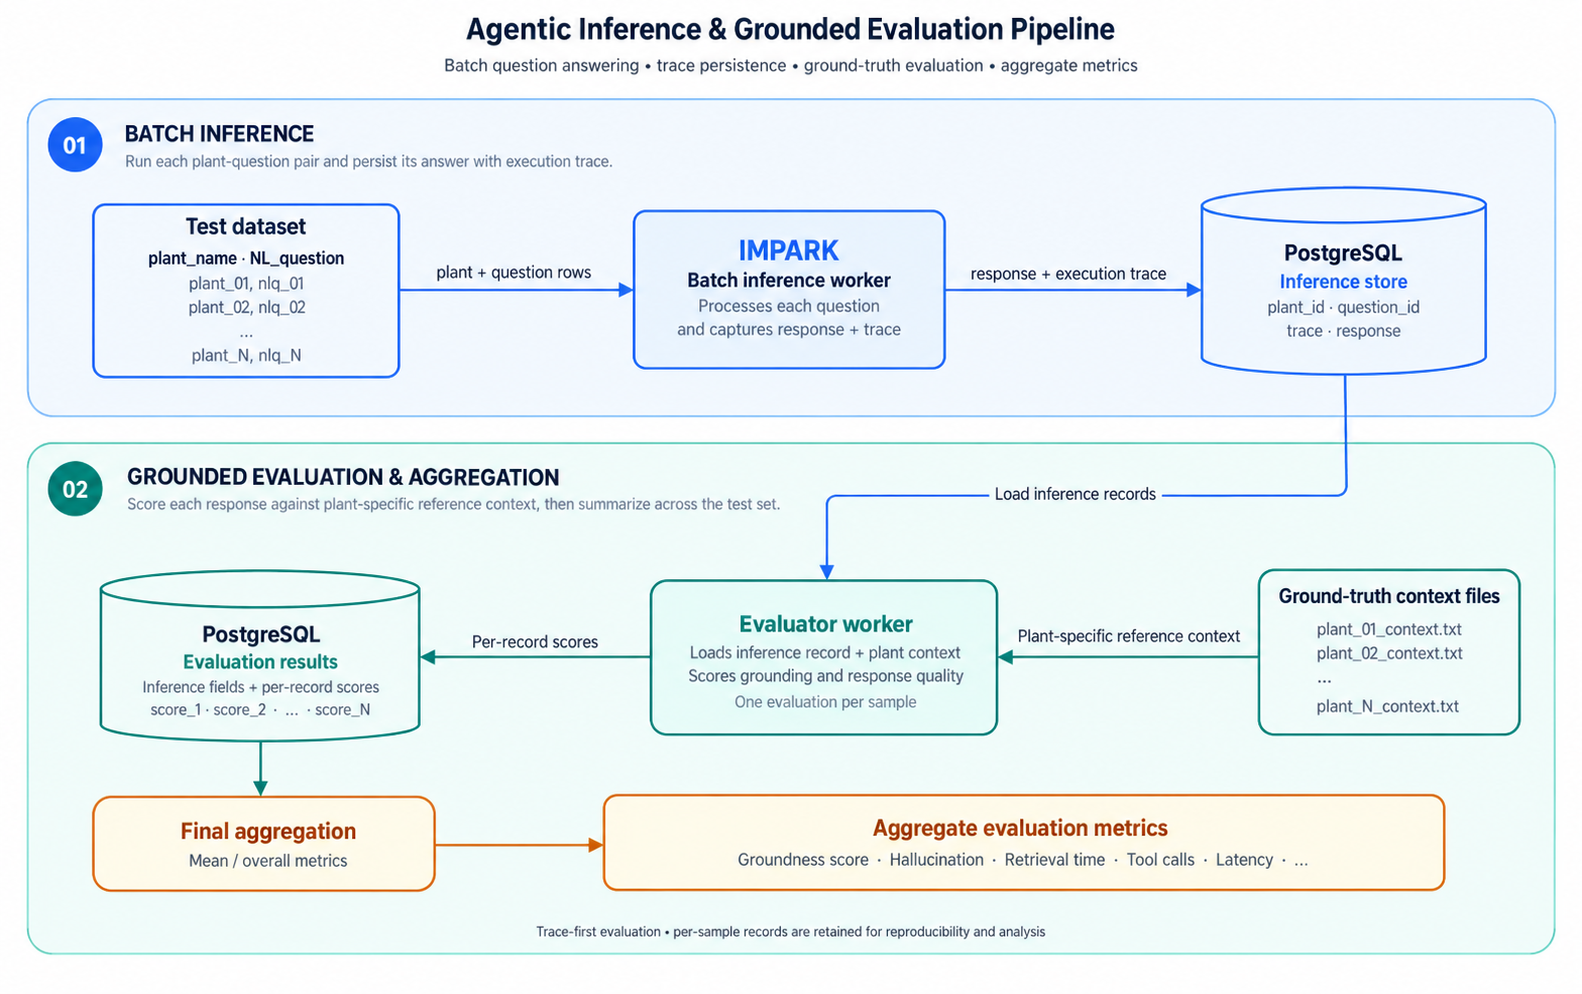
\includegraphics[width=0.88\textwidth]{figures/evaluation_workflow.png}
    \caption{Architecture of the automated evaluation pipeline.}
    \label{fig:eval_workflow}
\end{figure}

As illustrated in Figure~\ref{fig:eval_workflow}, the pipeline ingests execution traces from JSONL logs, slices canonical reference facts from bucket storage by query identifiers, segments candidate responses into atomic factual assertions, and validates each claim using dense embedding cosine similarity alongside normalized substring matching before recording metrics to PostgreSQL.

Performance is scored via Groundedness ($G$), Hallucination ($HR$), Tool Accuracy ($TCA$), and Latency ($T_{\text{graph}}$):
\begin{align}
G(\%) &= \frac{GC}{TGC} \times 100, \quad HR(\%) = 100\% - G(\%), \label{eq:groundedness} \\
TCA(\%) &= \frac{N_{\text{ok}}}{N_{\text{total}}} \times \omega_{\text{g}} \times 100, \quad T_{\text{graph}} = \sum_{m=1}^M \Delta t_{\text{dur}}\left(\tau^{(m)}\right). \label{eq:tca}
\end{align}

\section{Overall Performance and Analysis}

Figure~\ref{fig:dashboard_overview} shows the dashboard overview. Mean groundedness of 85.91\% exceeds zero-shot baselines, while 99.38\% tool accuracy confirms deterministic tool dispatch.

\begin{figure}[htbp]
    \centering
    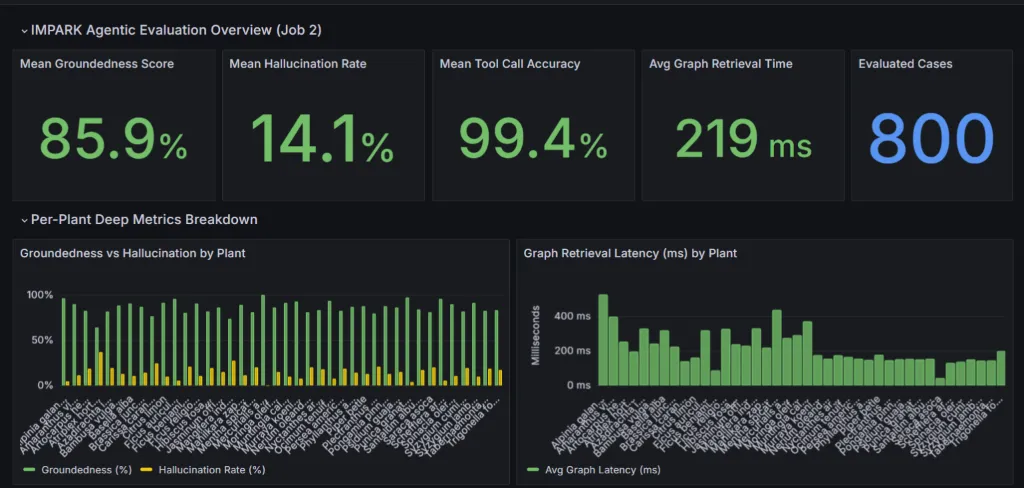
\includegraphics[width=0.92\textwidth]{figures/dashboard_overview_job2.png}
    \caption{Agentic Evaluation Dashboard overview for Job~2 over 800 test cases.}
    \label{fig:dashboard_overview}
\end{figure}

The dashboard interface in Figure~\ref{fig:dashboard_overview} highlights four top-level telemetry panels: Groundedness Score (85.9\%), Hallucination Rate (14.1\%), Tool Call Accuracy (99.4\%), and Knowledge Graph Latency (219~ms). Below the summary KPI cards, the console tracks real-time execution across the 800 evaluated cases, reporting claim verification rates, tool dispatch logs, and sub-second retrieval performance throughout the 455.45-second test execution.

Figure~\ref{fig:groundedness_chart} details Groundedness vs. Hallucination across all 40 taxa. Top taxa include \textit{Mercurialis annua} (100.0\%), \textit{Punica granatum} (96.9\%), \textit{Alpinia galanga} (96.1\%), and \textit{Ocimum tenuiflorum} (93.3\%). Sparsity lowered \textit{Atriplex hortensis} to 63.3\% (43 facts/20 queries).

\begin{figure}[htbp]
    \centering
    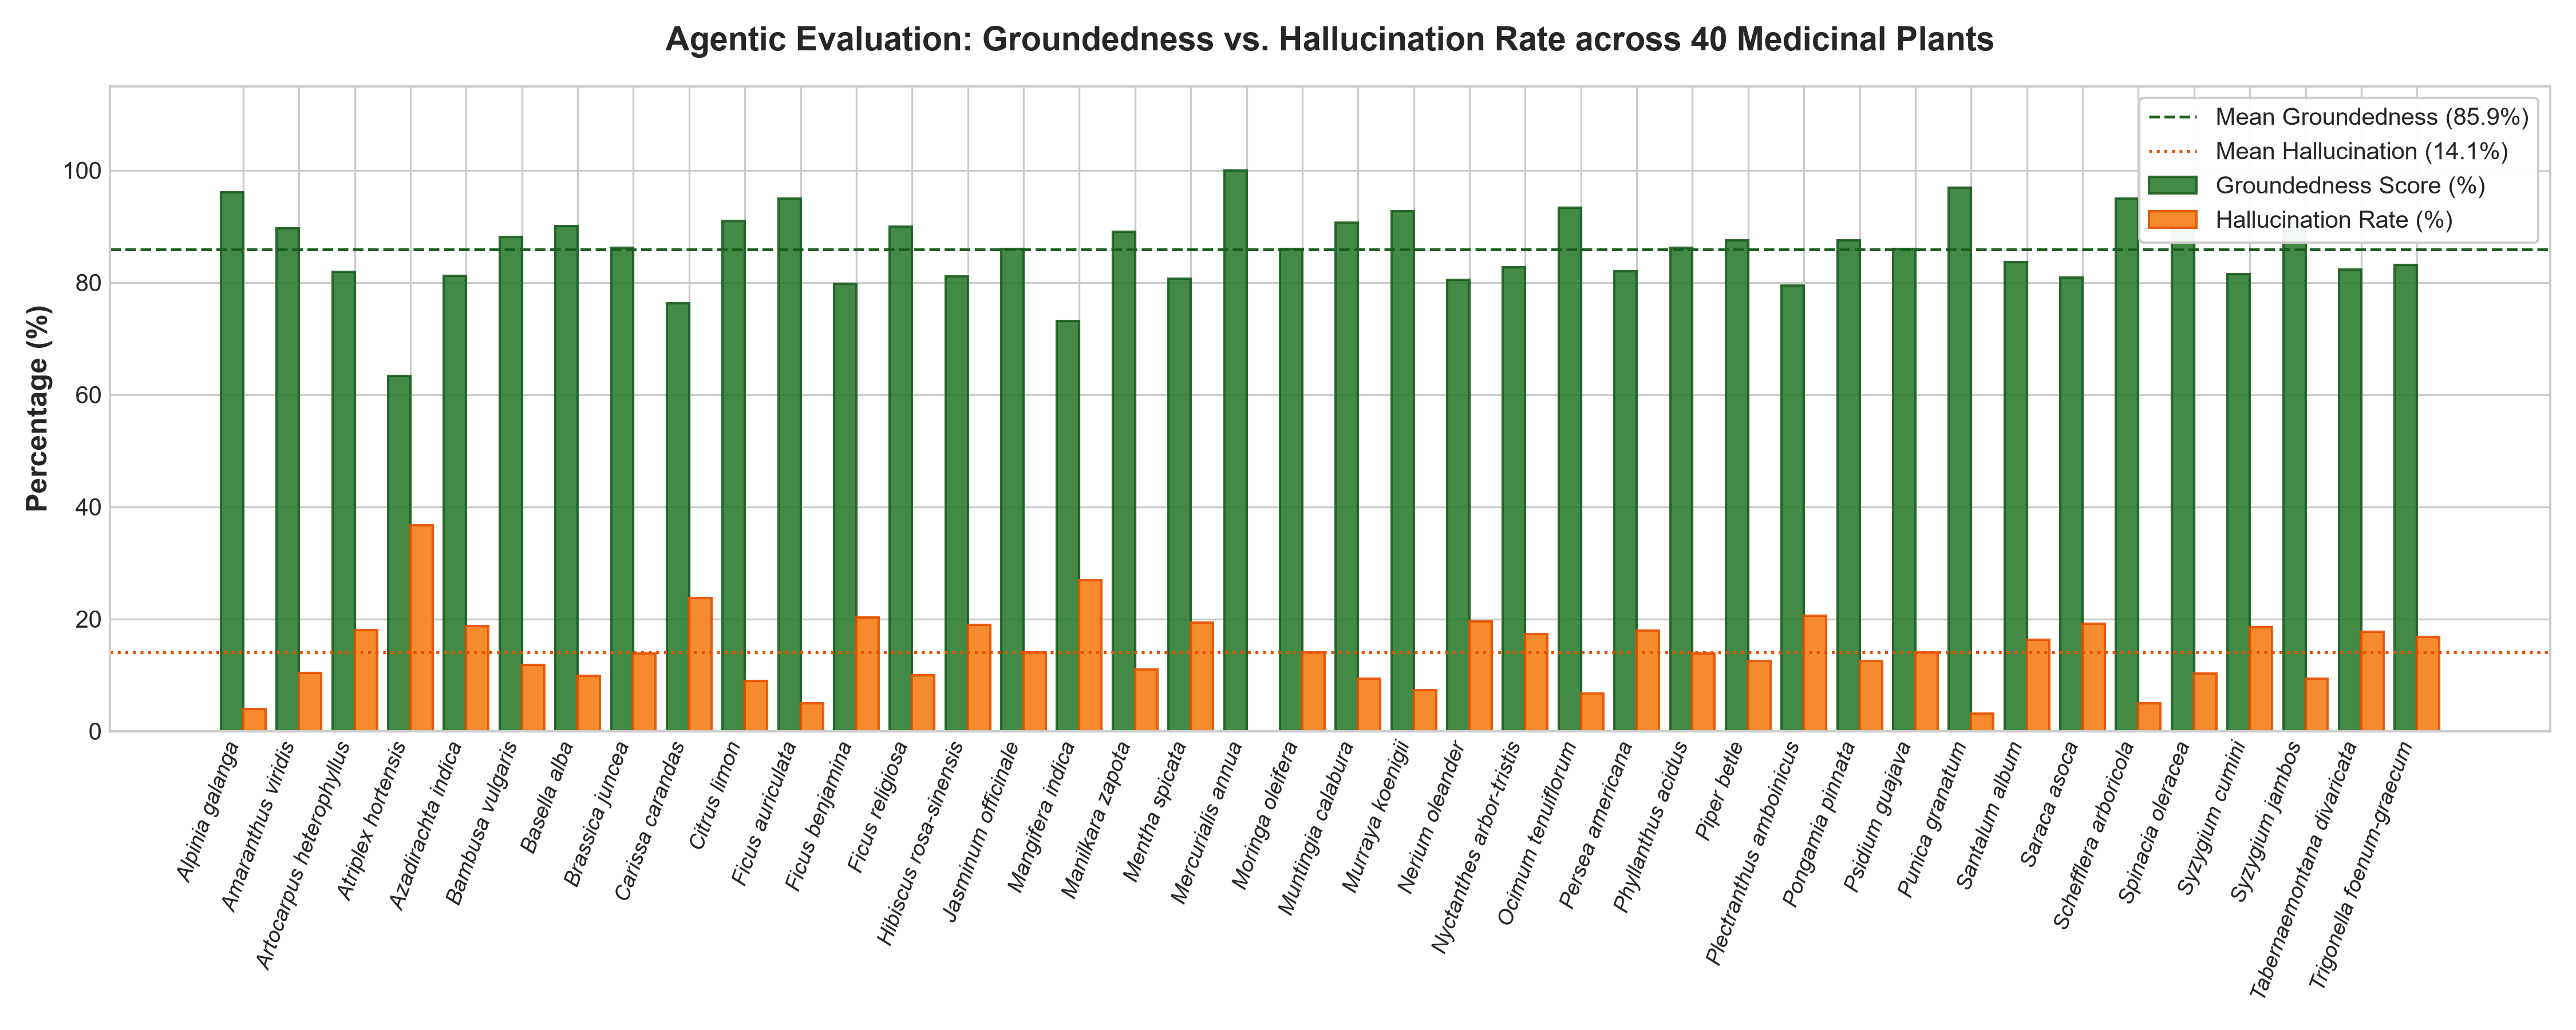
\includegraphics[width=0.90\textwidth]{figures/groundedness_hallucination_by_plant.png}
    \caption{Groundedness and Hallucination across all 40 species.}
    \label{fig:groundedness_chart}
\end{figure}

In Figure~\ref{fig:groundedness_chart}, the grouped bar chart contrasts Groundedness (green) against Hallucination Rate (orange) for each taxon alongside aggregate reference averages (dashed lines). Thirty-five of the forty species exceed 80\% groundedness, demonstrating consistent factual alignment across diverse plant families, with hallucinations concentrated in sparse taxa where missing graph entities prompted parametric generalization.

Latency averaged 218.52 ms (Figure~\ref{fig:latency_chart}), scaling from 40.4 ms (\textit{Saraca asoca}) to 528.5 ms (\textit{Alpinia galanga}).

\begin{figure}[htbp]
    \centering
    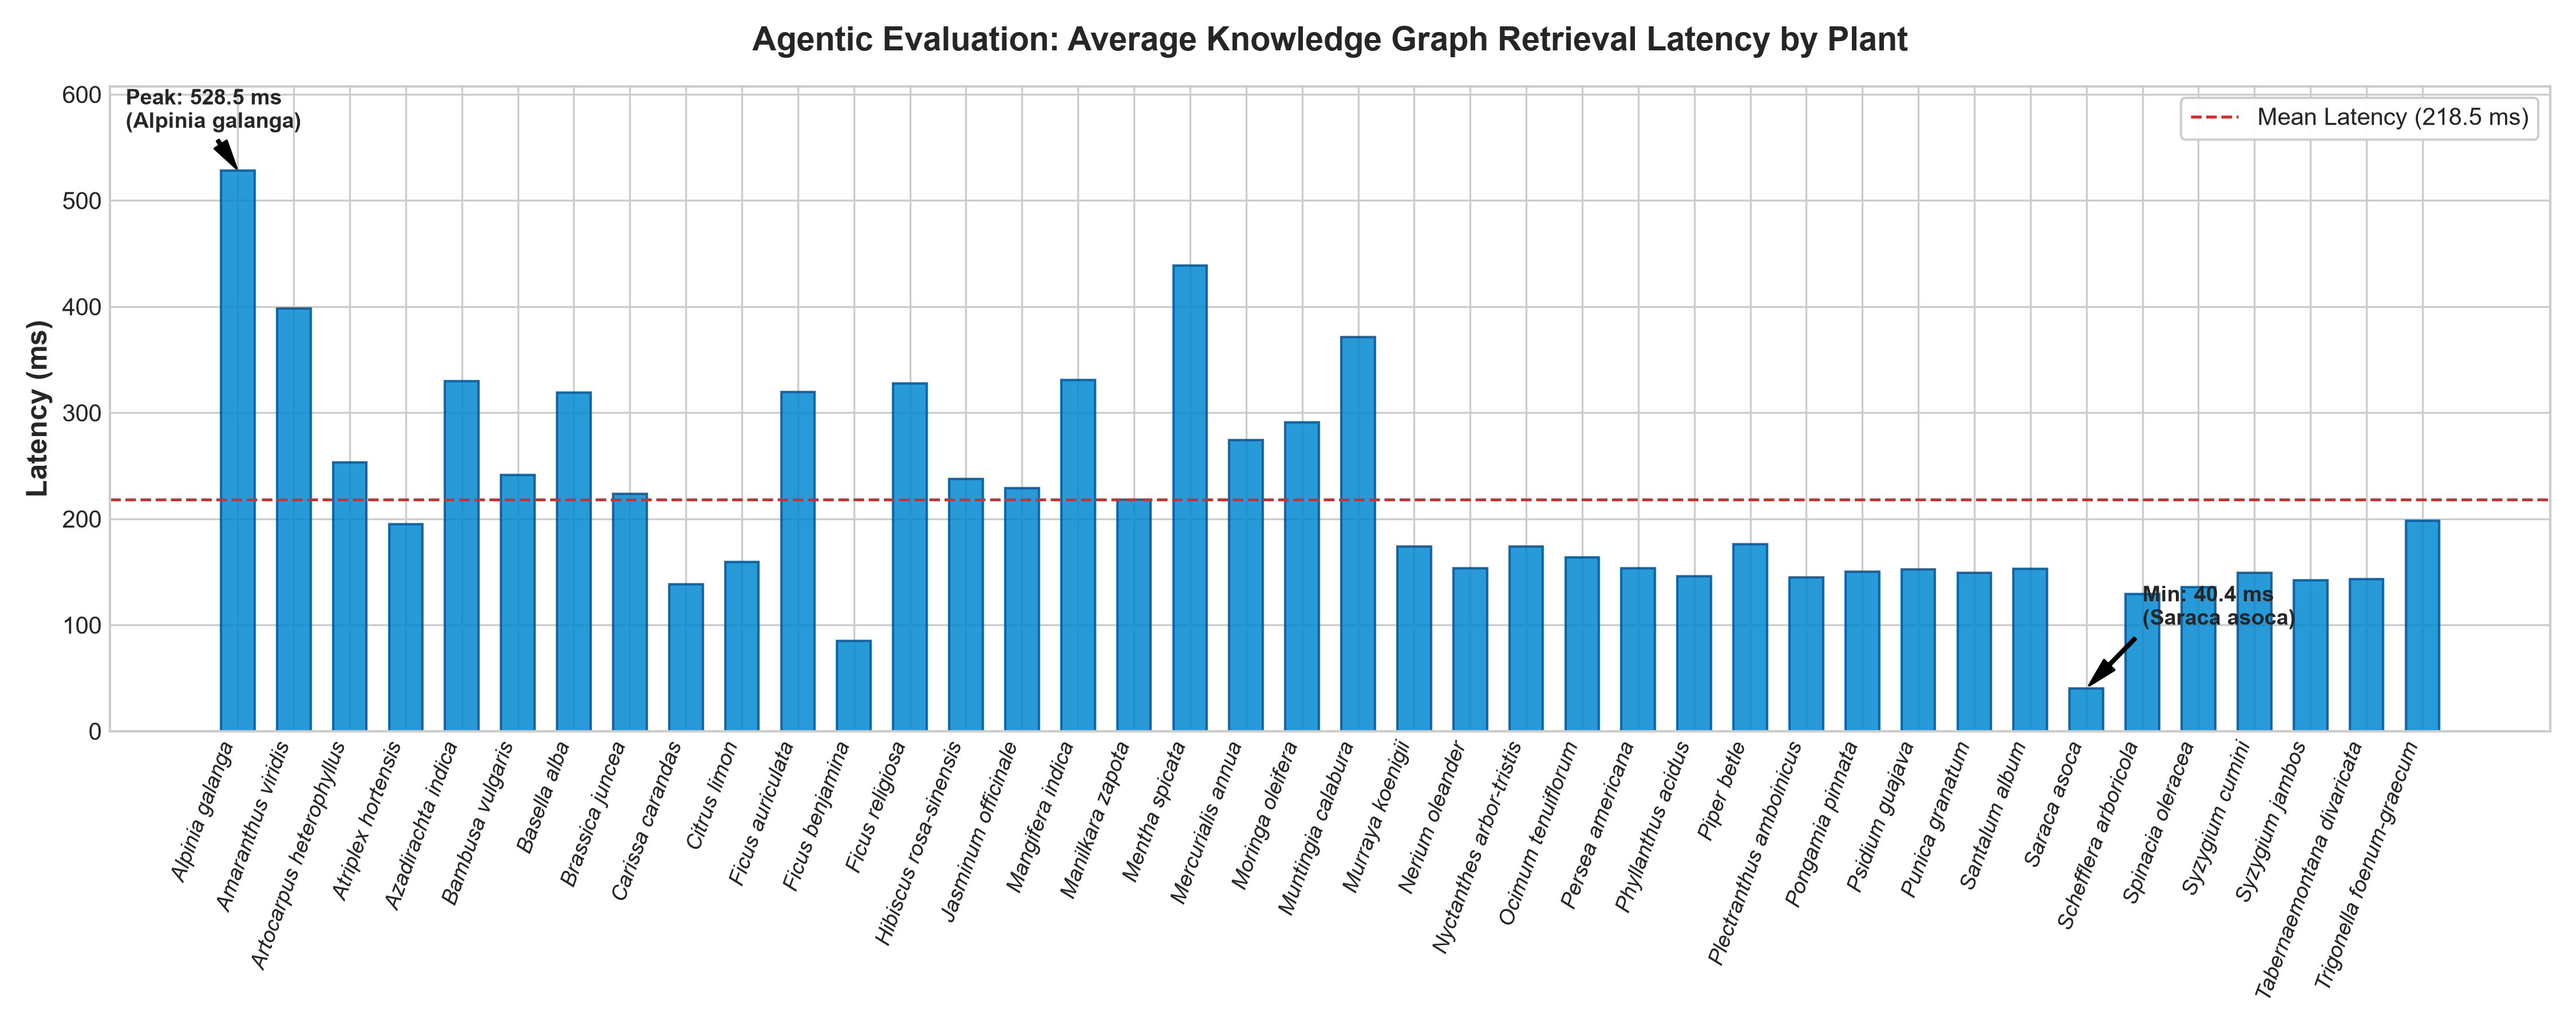
\includegraphics[width=0.92\textwidth]{figures/graph_retrieval_latency_by_plant.png}
    \caption{Average Knowledge Graph Retrieval Latency (ms) across all 40 medicinal plant species.}
    \label{fig:latency_chart}
\end{figure}

Figure~\ref{fig:latency_chart} plots knowledge graph retrieval duration per species relative to the 218.52~ms aggregate mean (red dashed line). Dense subgraphs with extensive phytochemical-protein relationships, such as \textit{Alpinia galanga} (528.5~ms) and \textit{Mentha spicata} (438.7~ms), incur higher multi-hop traversal costs, whereas compact single-hop structures like \textit{Saraca asoca} (40.4~ms) resolve rapidly, maintaining sub-second responsiveness across all 40 taxa.

\section{Per-Plant Performance Breakdown}

Table~\ref{tab:per_plant_breakdown} details experimental findings across all 40 evaluated plant taxa.

\begin{table}[htbp]
\centering
\scriptsize
\setlength{\tabcolsep}{2.5pt}
\caption{Comprehensive Evaluation Results across All 40 Indian Medicinal Plant Species (Job~2)}
\label{tab:per_plant_breakdown}
\begin{tabular}{@{}l c c c c c c c c@{}}
\hline
\textbf{Botanical Taxon Name} & \textbf{Cases} & \shortstack{\textbf{Grounded}\\\textbf{(\%)}} & \shortstack{\textbf{Halluc.}\\\textbf{(\%)}} & \shortstack{\textbf{Tool Acc.}\\\textbf{(\%)}} & \shortstack{\textbf{Latency}\\\textbf{(ms)}} & \shortstack{\textbf{Total}\\\textbf{Claims ($TGC$)}} & \shortstack{\textbf{Grounded}\\\textbf{Claims ($GC$)}} & \shortstack{\textbf{Halluc.}\\\textbf{Claims ($HC$)}} \\
\hline
\textit{Alpinia galanga} & 20 & 96.1\% & 3.9\% & 100.0\% & 528.5 & 196 & 185 & 11 \\
\textit{Amaranthus viridis} & 20 & 89.6\% & 10.4\% & 100.0\% & 398.4 & 131 & 126 & 5 \\
\textit{Artocarpus heterophyllus} & 20 & 81.9\% & 18.1\% & 100.0\% & 253.2 & 157 & 149 & 8 \\
\textit{Atriplex hortensis} & 20 & 63.3\% & 36.7\% & 100.0\% & 195.2 & 43 & 38 & 5 \\
\textit{Azadirachta indica} & 20 & 81.2\% & 18.8\% & 100.0\% & 330.0 & 171 & 162 & 9 \\
\textit{Bambusa vulgaris} & 20 & 88.2\% & 11.8\% & 100.0\% & 241.2 & 100 & 96 & 4 \\
\textit{Basella alba} & 20 & 90.1\% & 9.9\% & 100.0\% & 319.3 & 218 & 204 & 14 \\
\textit{Brassica juncea} & 20 & 86.2\% & 13.8\% & 100.0\% & 223.7 & 135 & 128 & 7 \\
\textit{Carissa carandas} & 20 & 76.3\% & 23.7\% & 100.0\% & 138.4 & 135 & 122 & 13 \\
\textit{Citrus limon} & 20 & 91.0\% & 9.0\% & 100.0\% & 159.7 & 192 & 184 & 8 \\
\textit{Ficus auriculata} & 20 & 95.0\% & 5.0\% & 100.0\% & 319.5 & 44 & 44 & 0 \\
\textit{Ficus benjamina} & 20 & 79.8\% & 20.2\% & 100.0\% & 85.0 & 73 & 62 & 11 \\
\textit{Ficus religiosa} & 20 & 90.0\% & 10.0\% & 100.0\% & 327.7 & 145 & 138 & 7 \\
\textit{Hibiscus rosa-sinensis} & 20 & 81.1\% & 18.9\% & 100.0\% & 237.9 & 179 & 170 & 9 \\
\textit{Jasminum officinale} & 20 & 85.9\% & 14.1\% & 100.0\% & 229.1 & 184 & 172 & 12 \\
\textit{Mangifera indica} & 20 & 73.1\% & 26.9\% & 100.0\% & 330.9 & 123 & 113 & 10 \\
\textit{Manilkara zapota} & 20 & 89.0\% & 11.0\% & 100.0\% & 218.0 & 158 & 146 & 12 \\
\textit{Mentha spicata} & 20 & 80.6\% & 19.4\% & 100.0\% & 438.7 & 125 & 118 & 7 \\
\textit{Mercurialis annua} & 20 & 100.0\% & 0.0\% & 100.0\% & 274.3 & 4 & 4 & 0 \\
\textit{Moringa oleifera} & 20 & 86.0\% & 14.0\% & 100.0\% & 291.1 & 185 & 169 & 16 \\
\textit{Muntingia calabura} & 20 & 90.7\% & 9.3\% & 100.0\% & 371.3 & 169 & 159 & 10 \\
\textit{Murraya koenigii} & 20 & 92.7\% & 7.3\% & 95.0\% & 174.1 & 159 & 154 & 5 \\
\textit{Nerium oleander} & 20 & 80.5\% & 19.5\% & 100.0\% & 153.3 & 156 & 145 & 11 \\
\textit{Nyctanthes arbor-tristis} & 20 & 82.7\% & 17.3\% & 100.0\% & 174.1 & 166 & 151 & 15 \\
\textit{Ocimum tenuiflorum} & 20 & 93.3\% & 6.7\% & 100.0\% & 163.5 & 208 & 195 & 13 \\
\textit{Persea americana} & 20 & 82.0\% & 18.0\% & 100.0\% & 153.7 & 113 & 106 & 7 \\
\textit{Phyllanthus acidus} & 20 & 86.2\% & 13.8\% & 95.0\% & 146.2 & 153 & 146 & 7 \\
\textit{Piper betle} & 20 & 87.5\% & 12.5\% & 100.0\% & 176.1 & 181 & 175 & 6 \\
\textit{Plectranthus amboinicus} & 20 & 79.4\% & 20.6\% & 95.0\% & 144.9 & 116 & 105 & 11 \\
\textit{Pongamia pinnata} & 20 & 87.5\% & 12.5\% & 100.0\% & 150.4 & 154 & 147 & 7 \\
\textit{Psidium guajava} & 20 & 86.0\% & 14.0\% & 100.0\% & 152.4 & 134 & 125 & 9 \\
\textit{Punica granatum} & 20 & 96.9\% & 3.1\% & 100.0\% & 149.3 & 203 & 195 & 8 \\
\textit{Santalum album} & 20 & 83.7\% & 16.3\% & 100.0\% & 153.2 & 153 & 140 & 13 \\
\textit{Saraca asoca} & 20 & 80.8\% & 19.2\% & 100.0\% & 40.4 & 134 & 123 & 11 \\
\textit{Schefflera arboricola} & 20 & 95.0\% & 5.0\% & 95.0\% & 129.5 & 5 & 5 & 0 \\
\textit{Spinacia oleracea} & 20 & 89.7\% & 10.3\% & 100.0\% & 135.6 & 188 & 173 & 15 \\
\textit{Syzygium cumini} & 20 & 81.5\% & 18.5\% & 100.0\% & 149.0 & 124 & 115 & 9 \\
\textit{Syzygium jambos} & 20 & 90.6\% & 9.4\% & 100.0\% & 142.5 & 181 & 165 & 16 \\
\textit{Tabernaemontana divaricata} & 20 & 82.3\% & 17.7\% & 100.0\% & 143.4 & 168 & 161 & 7 \\
\textit{Trigonella foenum-graecum} & 20 & 83.1\% & 16.9\% & 95.0\% & 198.3 & 152 & 140 & 12 \\
\hline
\textbf{Overall System Aggregate} & \textbf{800} & \textbf{85.9\%} & \textbf{14.1\%} & \textbf{99.4\%} & \textbf{218.5} & \textbf{5,715} & \textbf{5,355} & \textbf{360} \\
\hline
\end{tabular}
\end{table}

\section{Discussion and Limitations}

Parameterized Cypher bounds answer synthesis to verified graph nodes, reducing hallucination to 14.09\%. Dual-boundary semantic verification balances linguistic paraphrasing with string fidelity. The framework is an academic demonstration system and not a clinical diagnostic or treatment tool.
